\documentclass[11pt]{article}
\usepackage[margin=0.7in]{geometry}
\usepackage{multirow}
\usepackage {graphicx}
\usepackage[utf8x]{inputenc} % указать кодировку русского текста
\usepackage[russian]{babel} % указать, что язык текста - русский
\usepackage{fancyhdr}
\pagestyle{fancy}
\begin{document}
\begin{titlepage}
\begin{center}
%\vspace*{1cm}
\large\textbf{Московский Физико-Технический Институт}\\
\large\textbf{(государственный университет)}
\vfill
\line(1,0){430}\\[1mm]
\huge\textbf{Исследование взаимной диффузии газов}\\
\line(1,0){430}\\[1mm]
\vfill
\large ФОПФ\\
\end{center}
\end{titlepage}
\fancyhead[L] {Работа 2.2.1}
\noindent \textbf{Цель работы:} \\
\indent 1)  регистрация  зависимости  концентрации   гелия в воздухе от времени с помощью датчиков теплопроводности при разных начальных давлениях смеси газов; 2) определение коэффициента диффузии по результатам измерений.\\
\noindent \textbf{В работе используются:} \\
\indent измерительная установка; форвакуумный насос; баллон с газом (гелий); манометр; источник питания; магазин сопротивлений; гальванометр; секундомер.
\section*{Описание работы}\
\indent Рассмотрим процесс выравнивания концентрации. Закон Фика:
$$j=-D\frac{\partial n}{\partial x}$$
В нашем случае ввиду того что, а) объем соединительной трубки мал по сравнению с объемами сосудов, б) концентрацию газов внутри каждого сосуда можно считать постоянной по всему объему.
$$J=-DS\frac{n_1-n_2}{l}$$
Изменение компонента в сосудах: $V_1\Delta n_1=-V_2\Delta n_2$\\
\ \\
С другой стороны $V_1\Delta n_1=J\Delta t$ и $V_1\frac{dn_1}{dt}=-DS\frac{n_1-n_2}{l}$; \ \ \  Аналогично $V_2\frac{dn_2}{dt}=DS\frac{n_1-n_2}{l}$\\
\ \\
Тогда $$\frac{d(n_1-n_2)}{dt}=-\frac{n_1-n_2}{l} \frac{V_1+V_2}{V_1V_2}$$
Проинтегрируем и получим, что
$$n_1-n_2=(n_1-n_2)_0 e^{-t/\tau}, \tau=\frac{V_1V_2}{V_1+V_2}\frac{l}{SD}=/V_1=V_2=V/=\frac{Vl}{2SD}$$\\
 При заполнении сосудов смесями различного состава возникает «разбаланc» моста. При незначительном различии в составах смесей показания гальванометра, подсоединённого к диагонали моста, будут пропорциональны разности концентраций примеси. В процессе диффузии
разность концентраций убывает по экспоненте, и значит по тому же закону изменяются во времени показания гальванометра
$$U=U_0 \exp(-t/\tau)$$
\section*{Оборудование}\
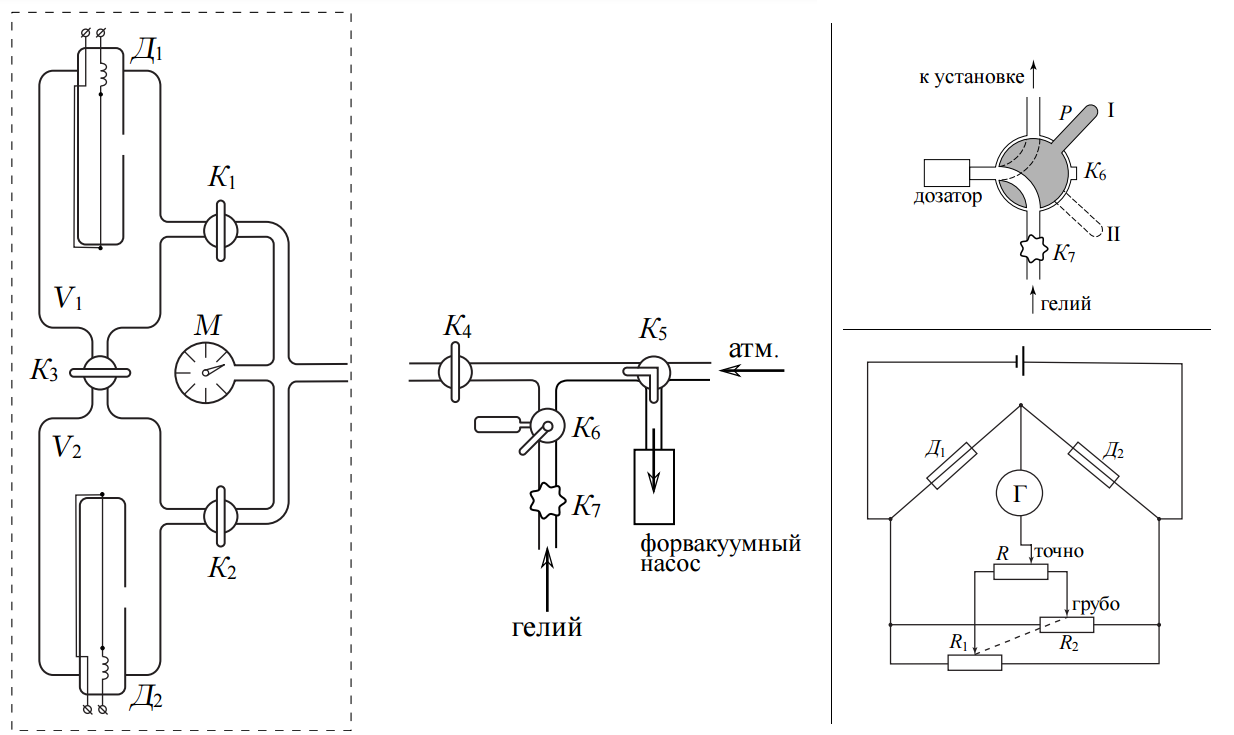
\includegraphics[scale=0.4]{pic1.png}
\section*{Ход работы}\
Перепишем параметры установки:\\
$V=(1200\pm 30)$ см$^3$;\ \ $l/s=(5,5\pm 0,5)$ см$^{-1}$; \\
Тогда постоянная установки $M=(3300\pm 300)$ см$^2$\\
Рабочие давления: $P_{He}=0,2P_{rab}$; \ \ \ $P_{Air}=1,75P_{rab}$\\
\ \\
\textbf{Таблицы значений:}\\
\ \\
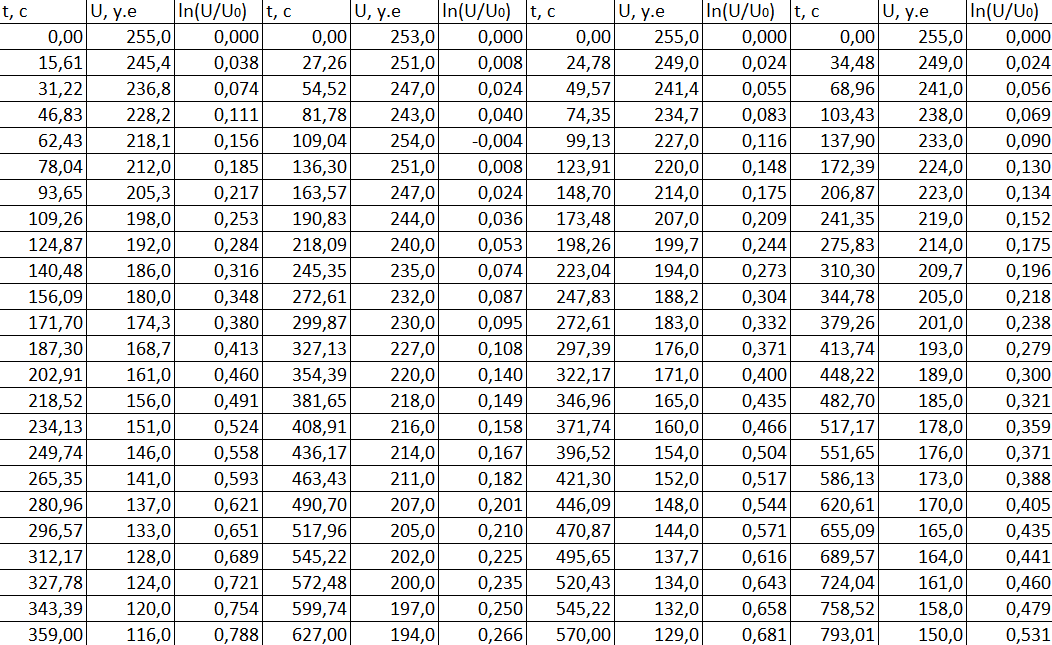
\includegraphics[scale=0.8]{table.png}\\
\ \\
\newpage
\textbf{Графики:}\\
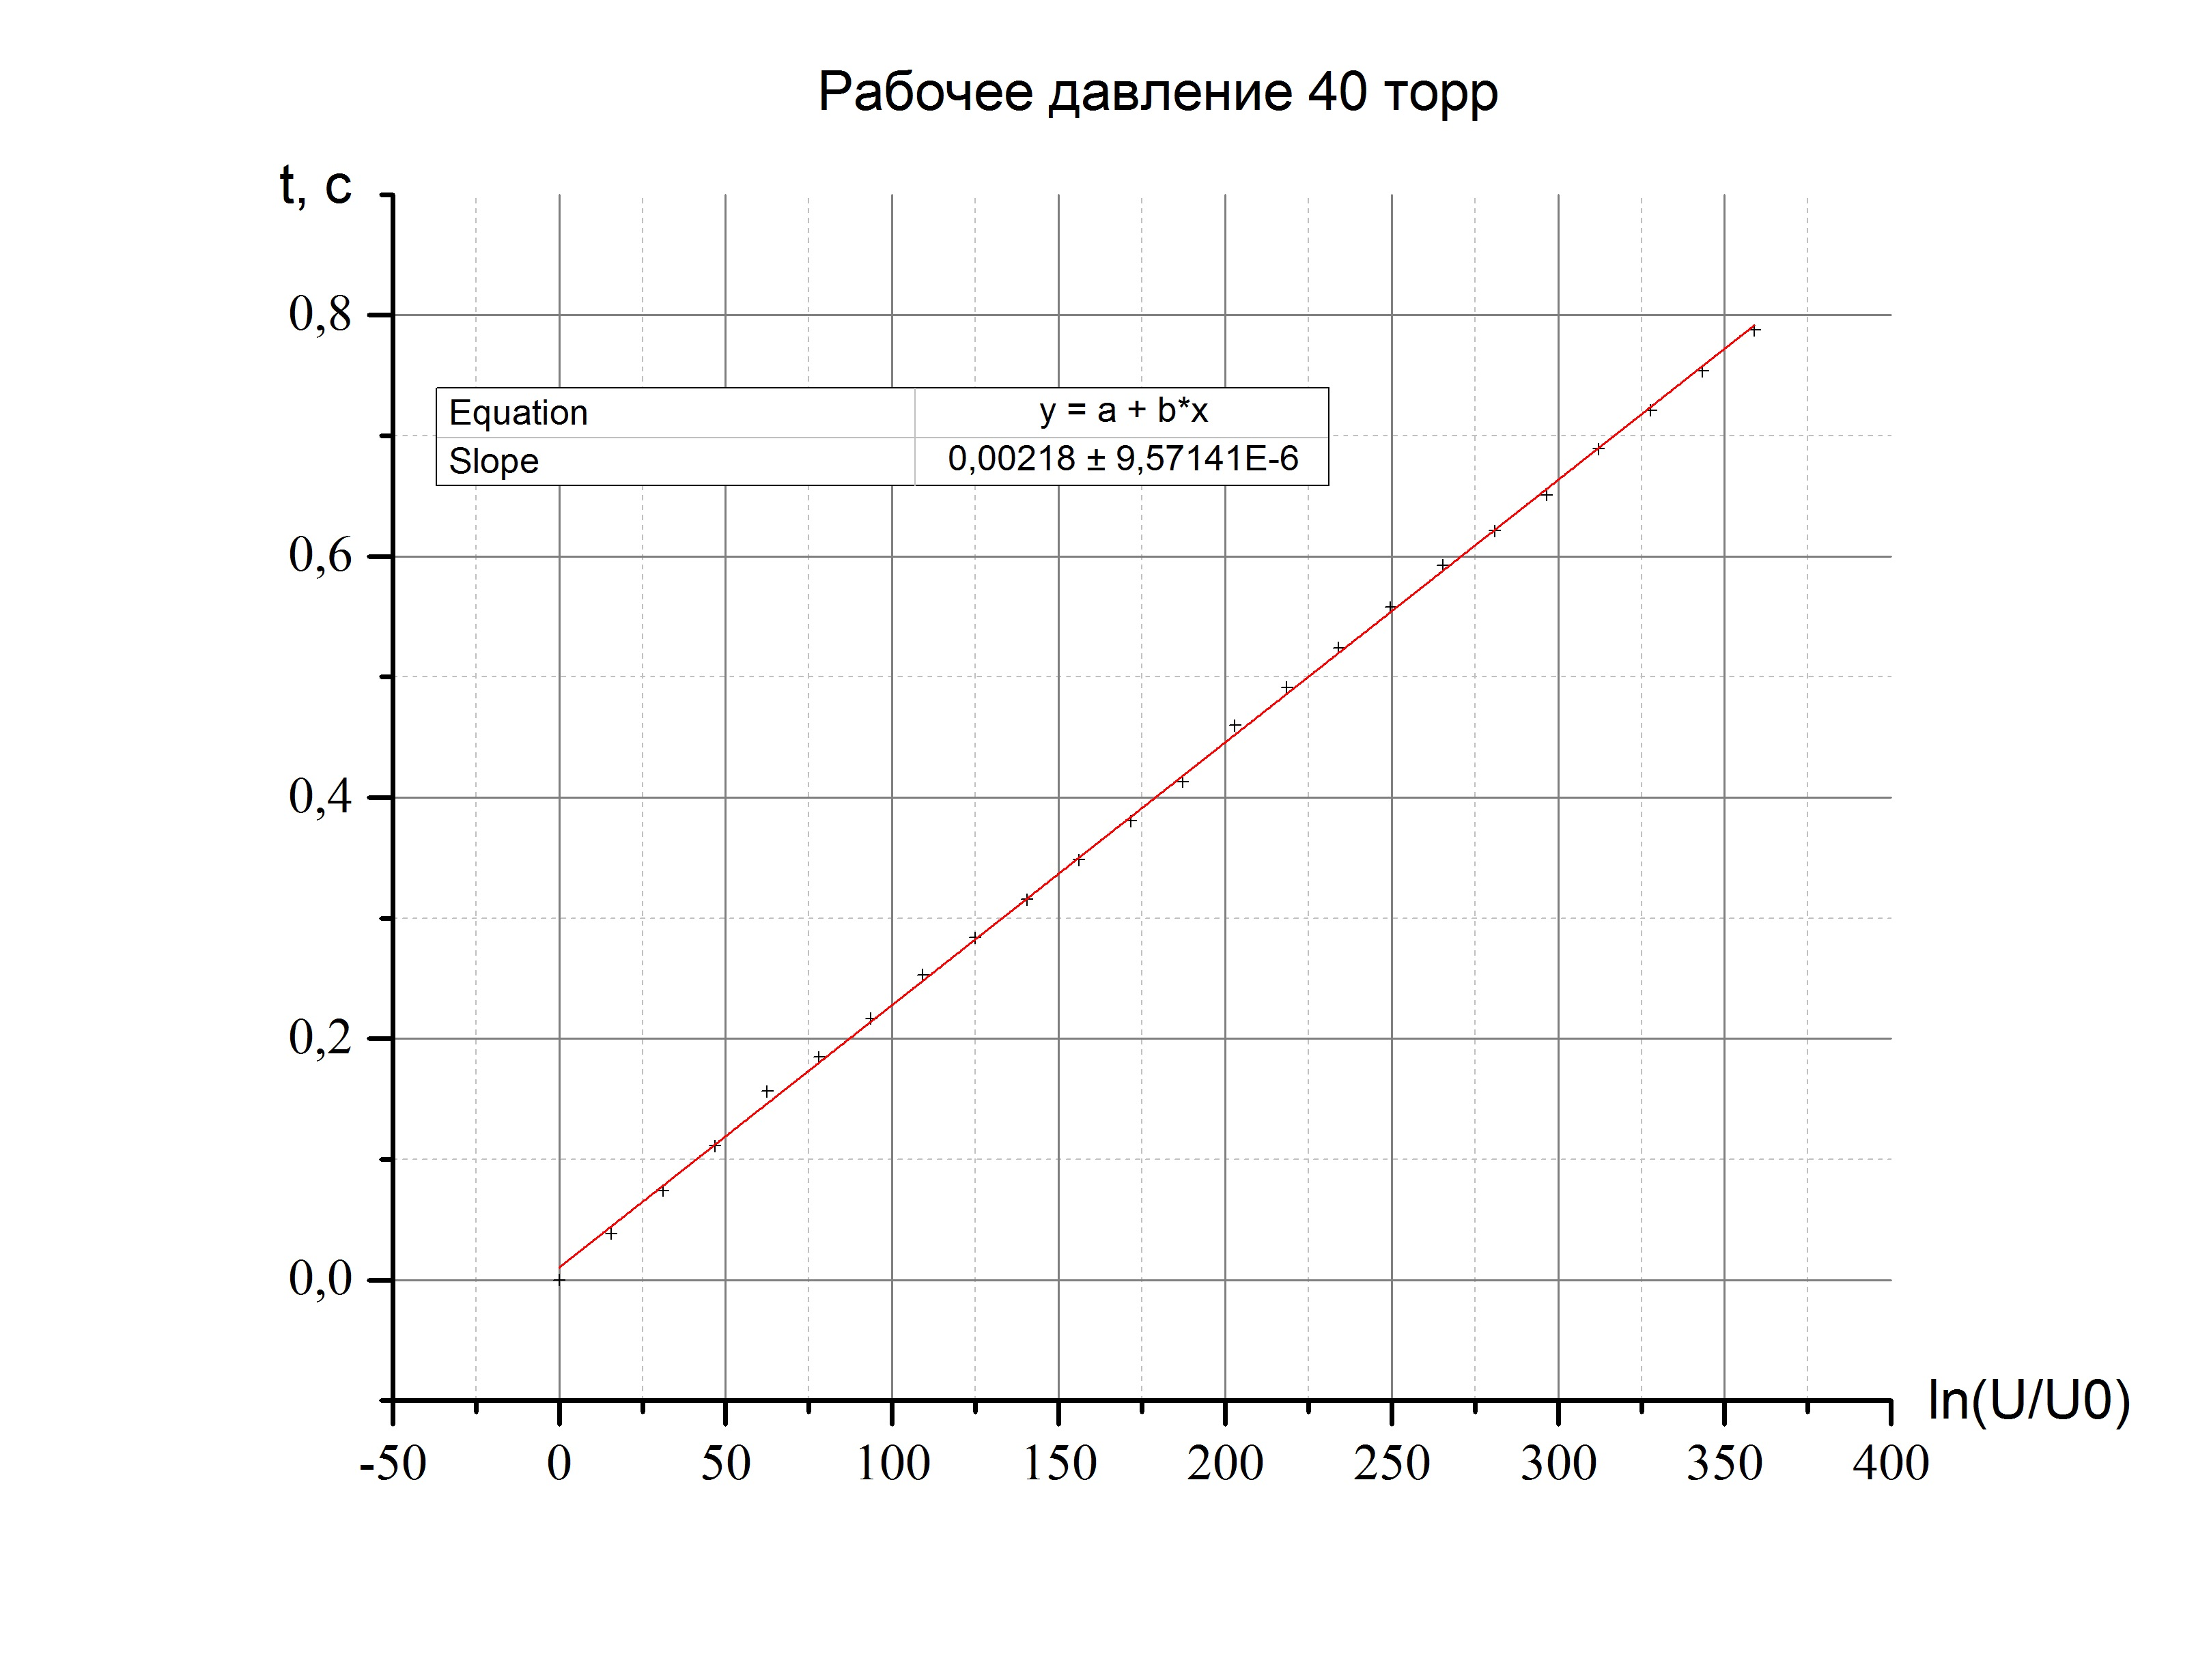
\includegraphics[scale=0.55]{Graph5.jpg}\\
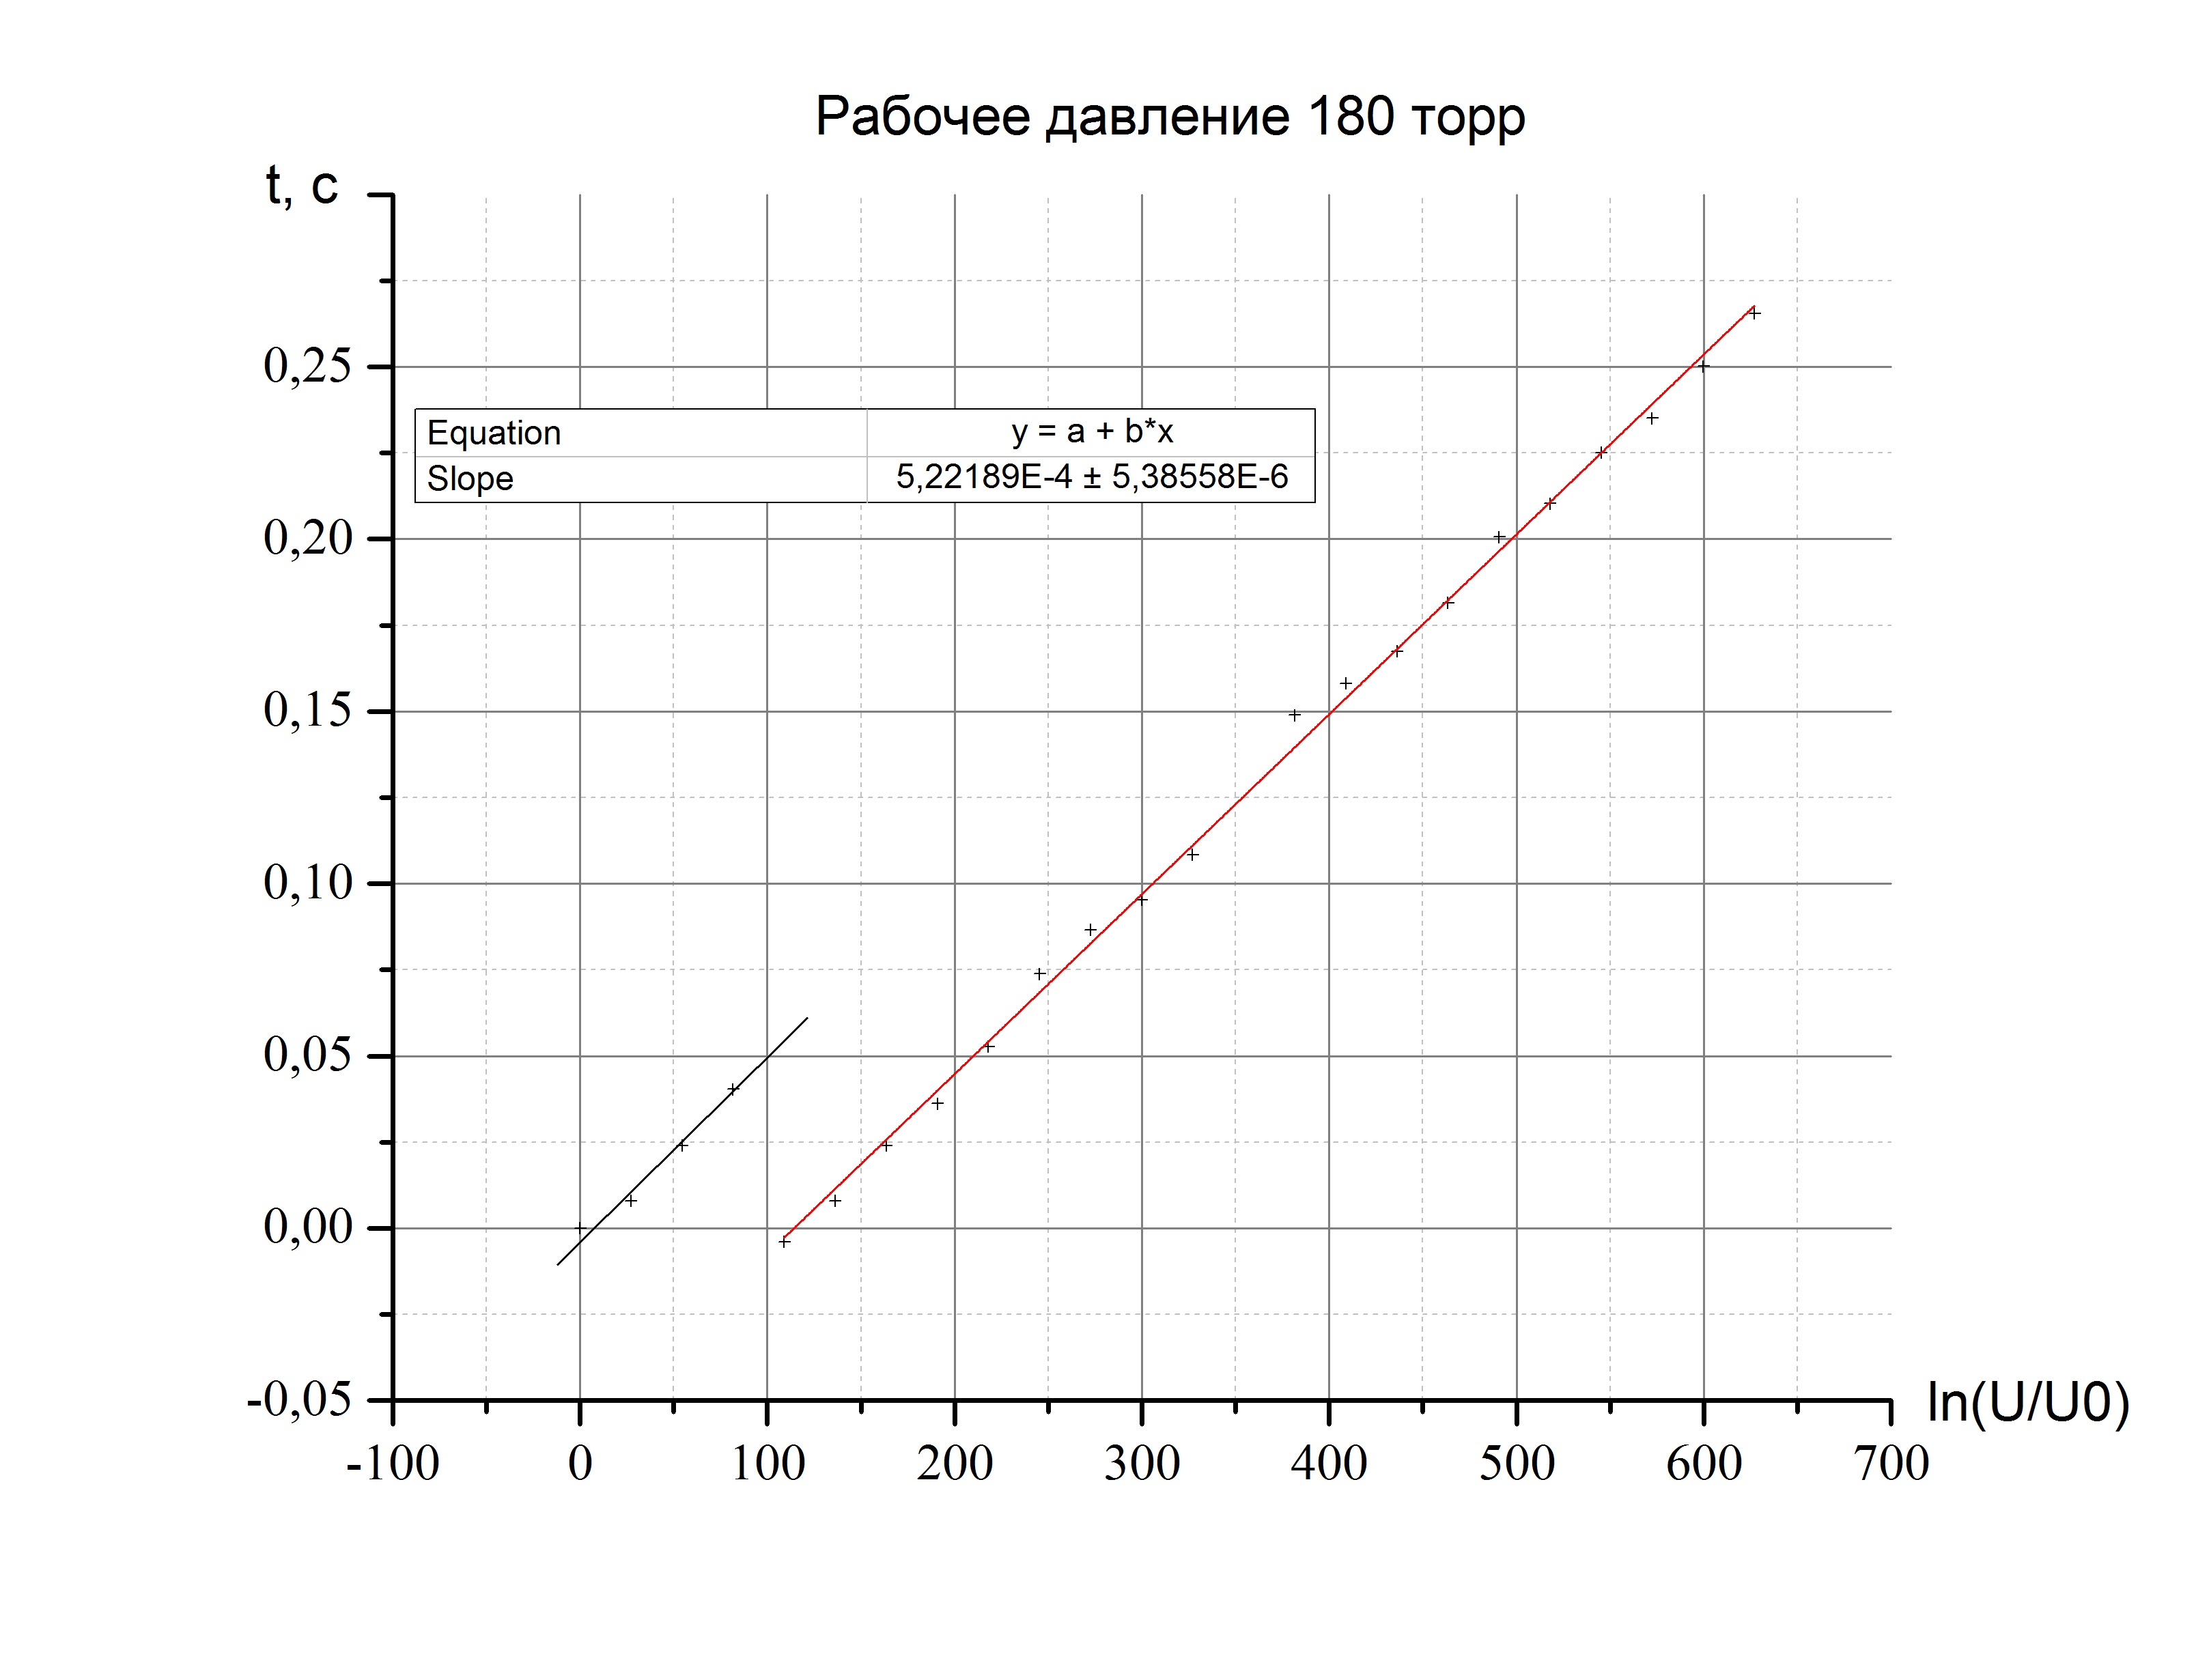
\includegraphics[scale=0.55]{Graph6.jpg}\\
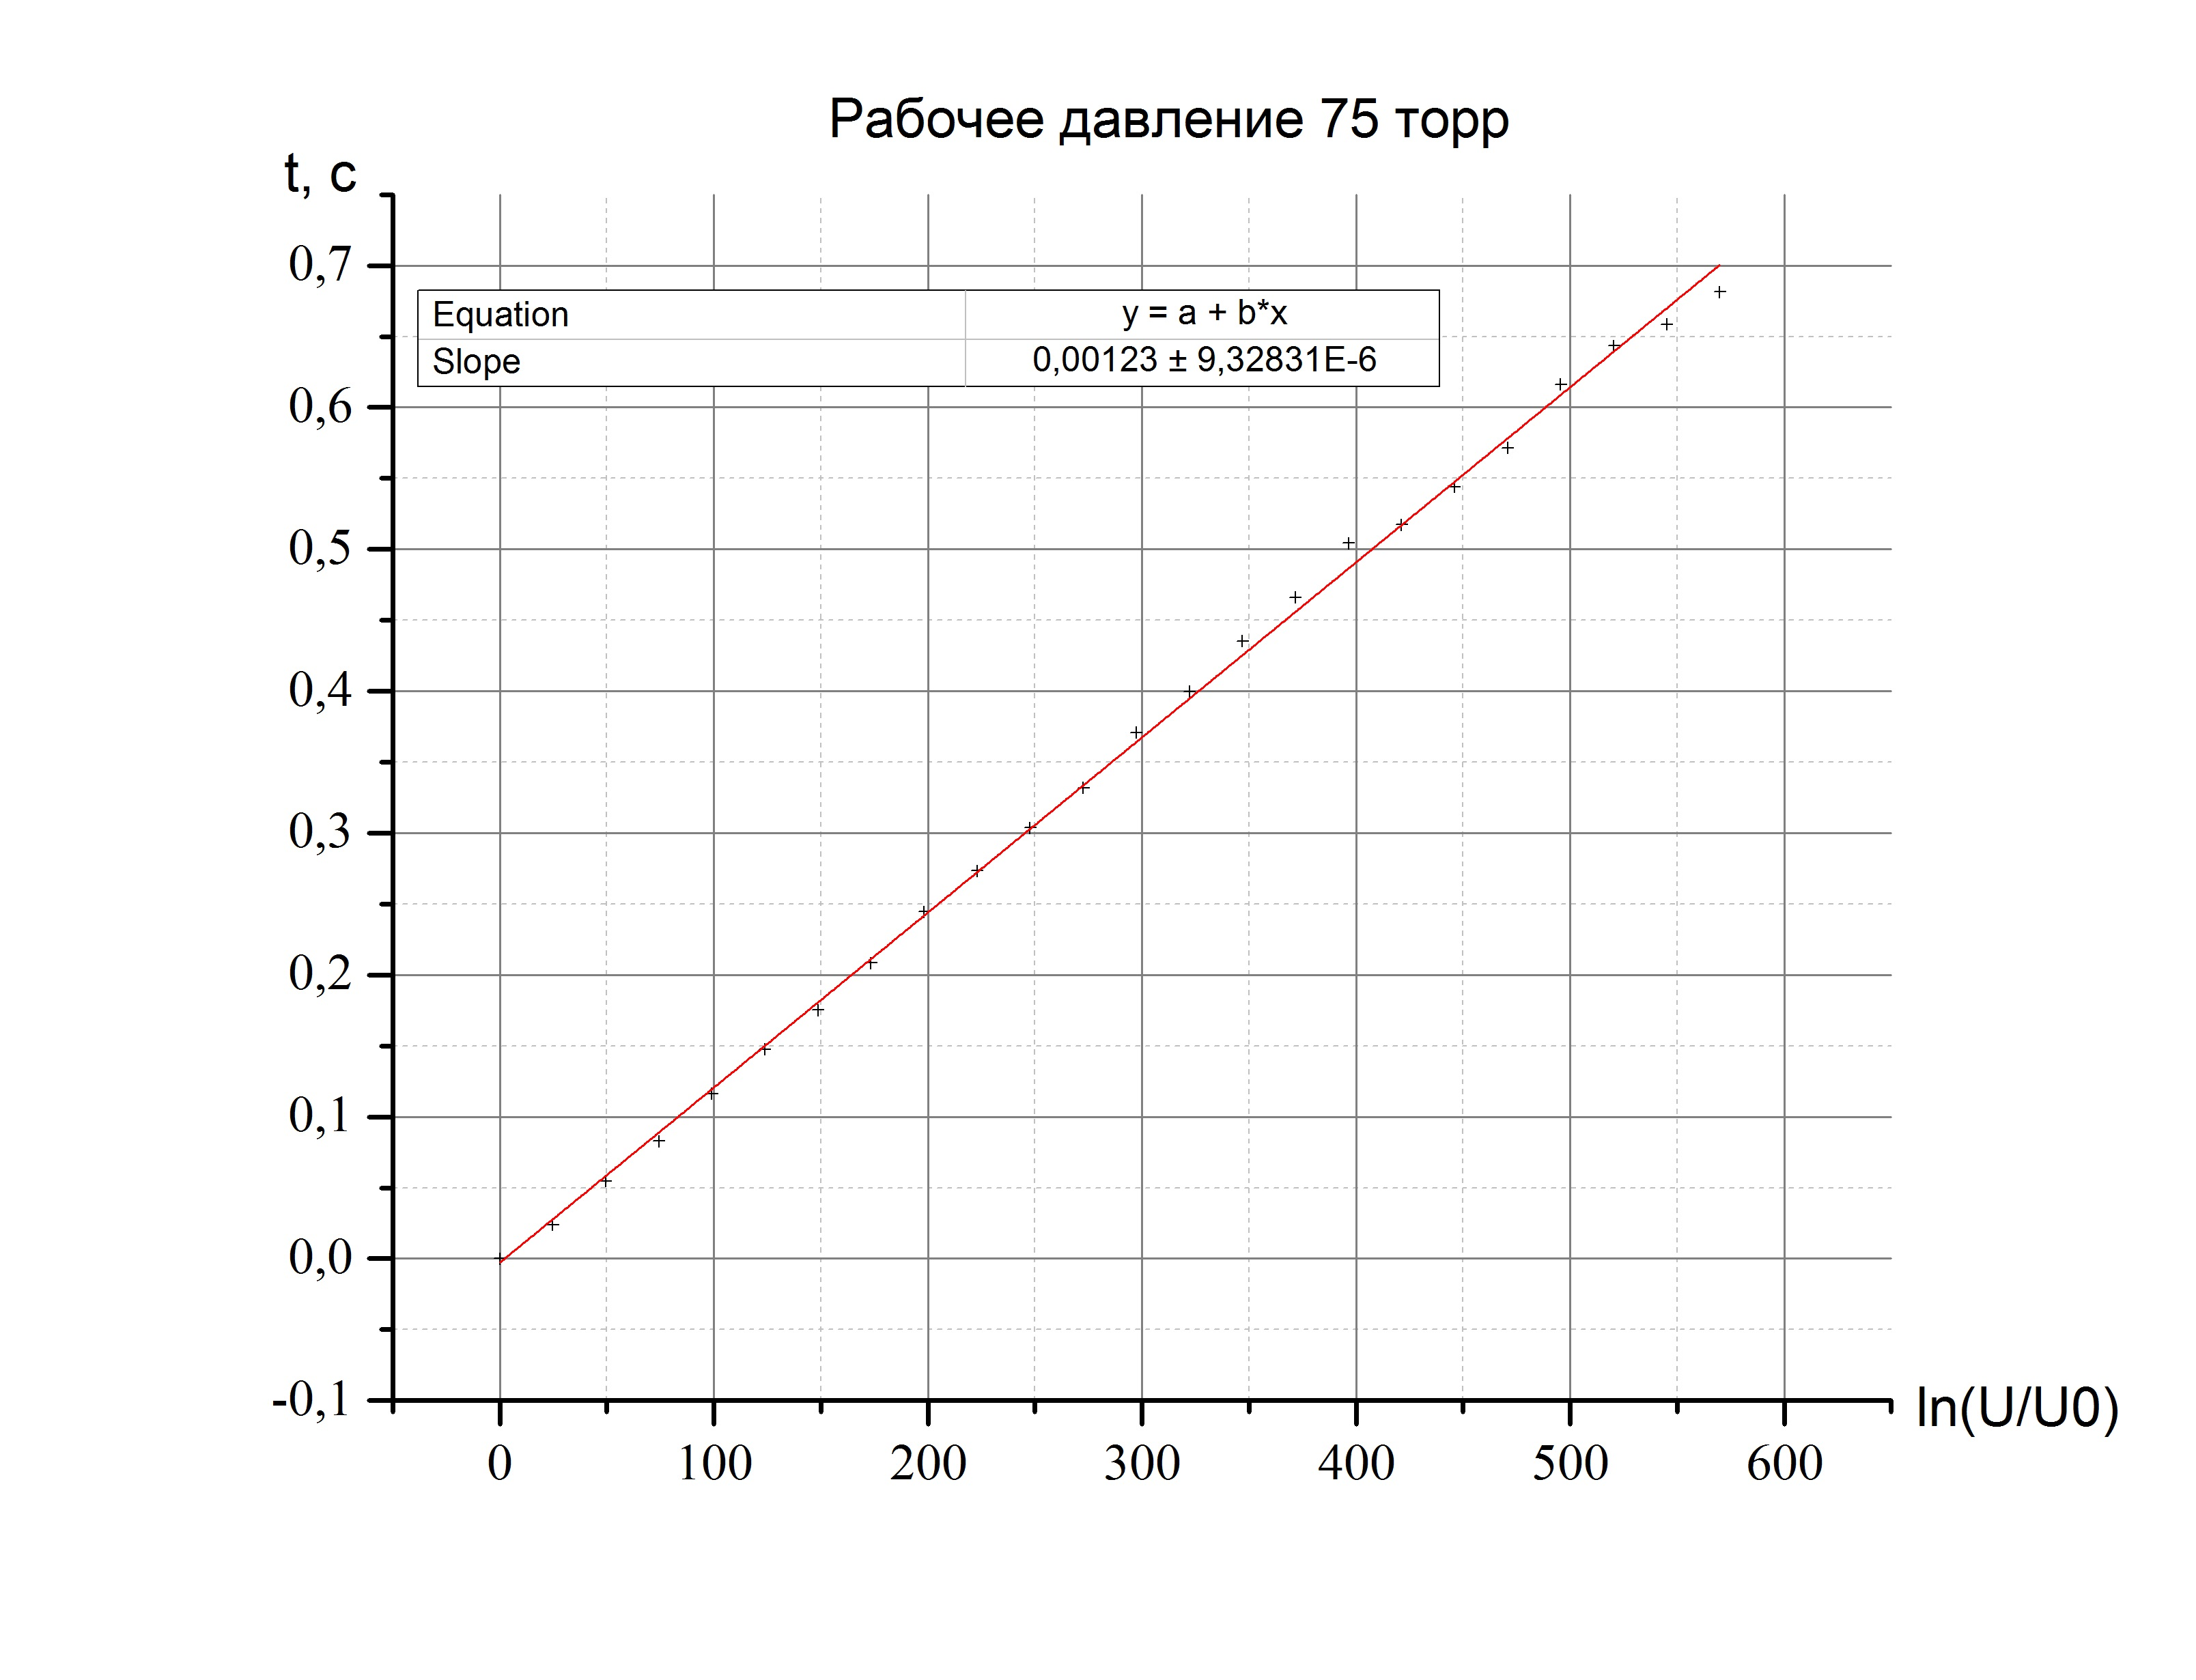
\includegraphics[scale=0.55]{Graph7.jpg}\\
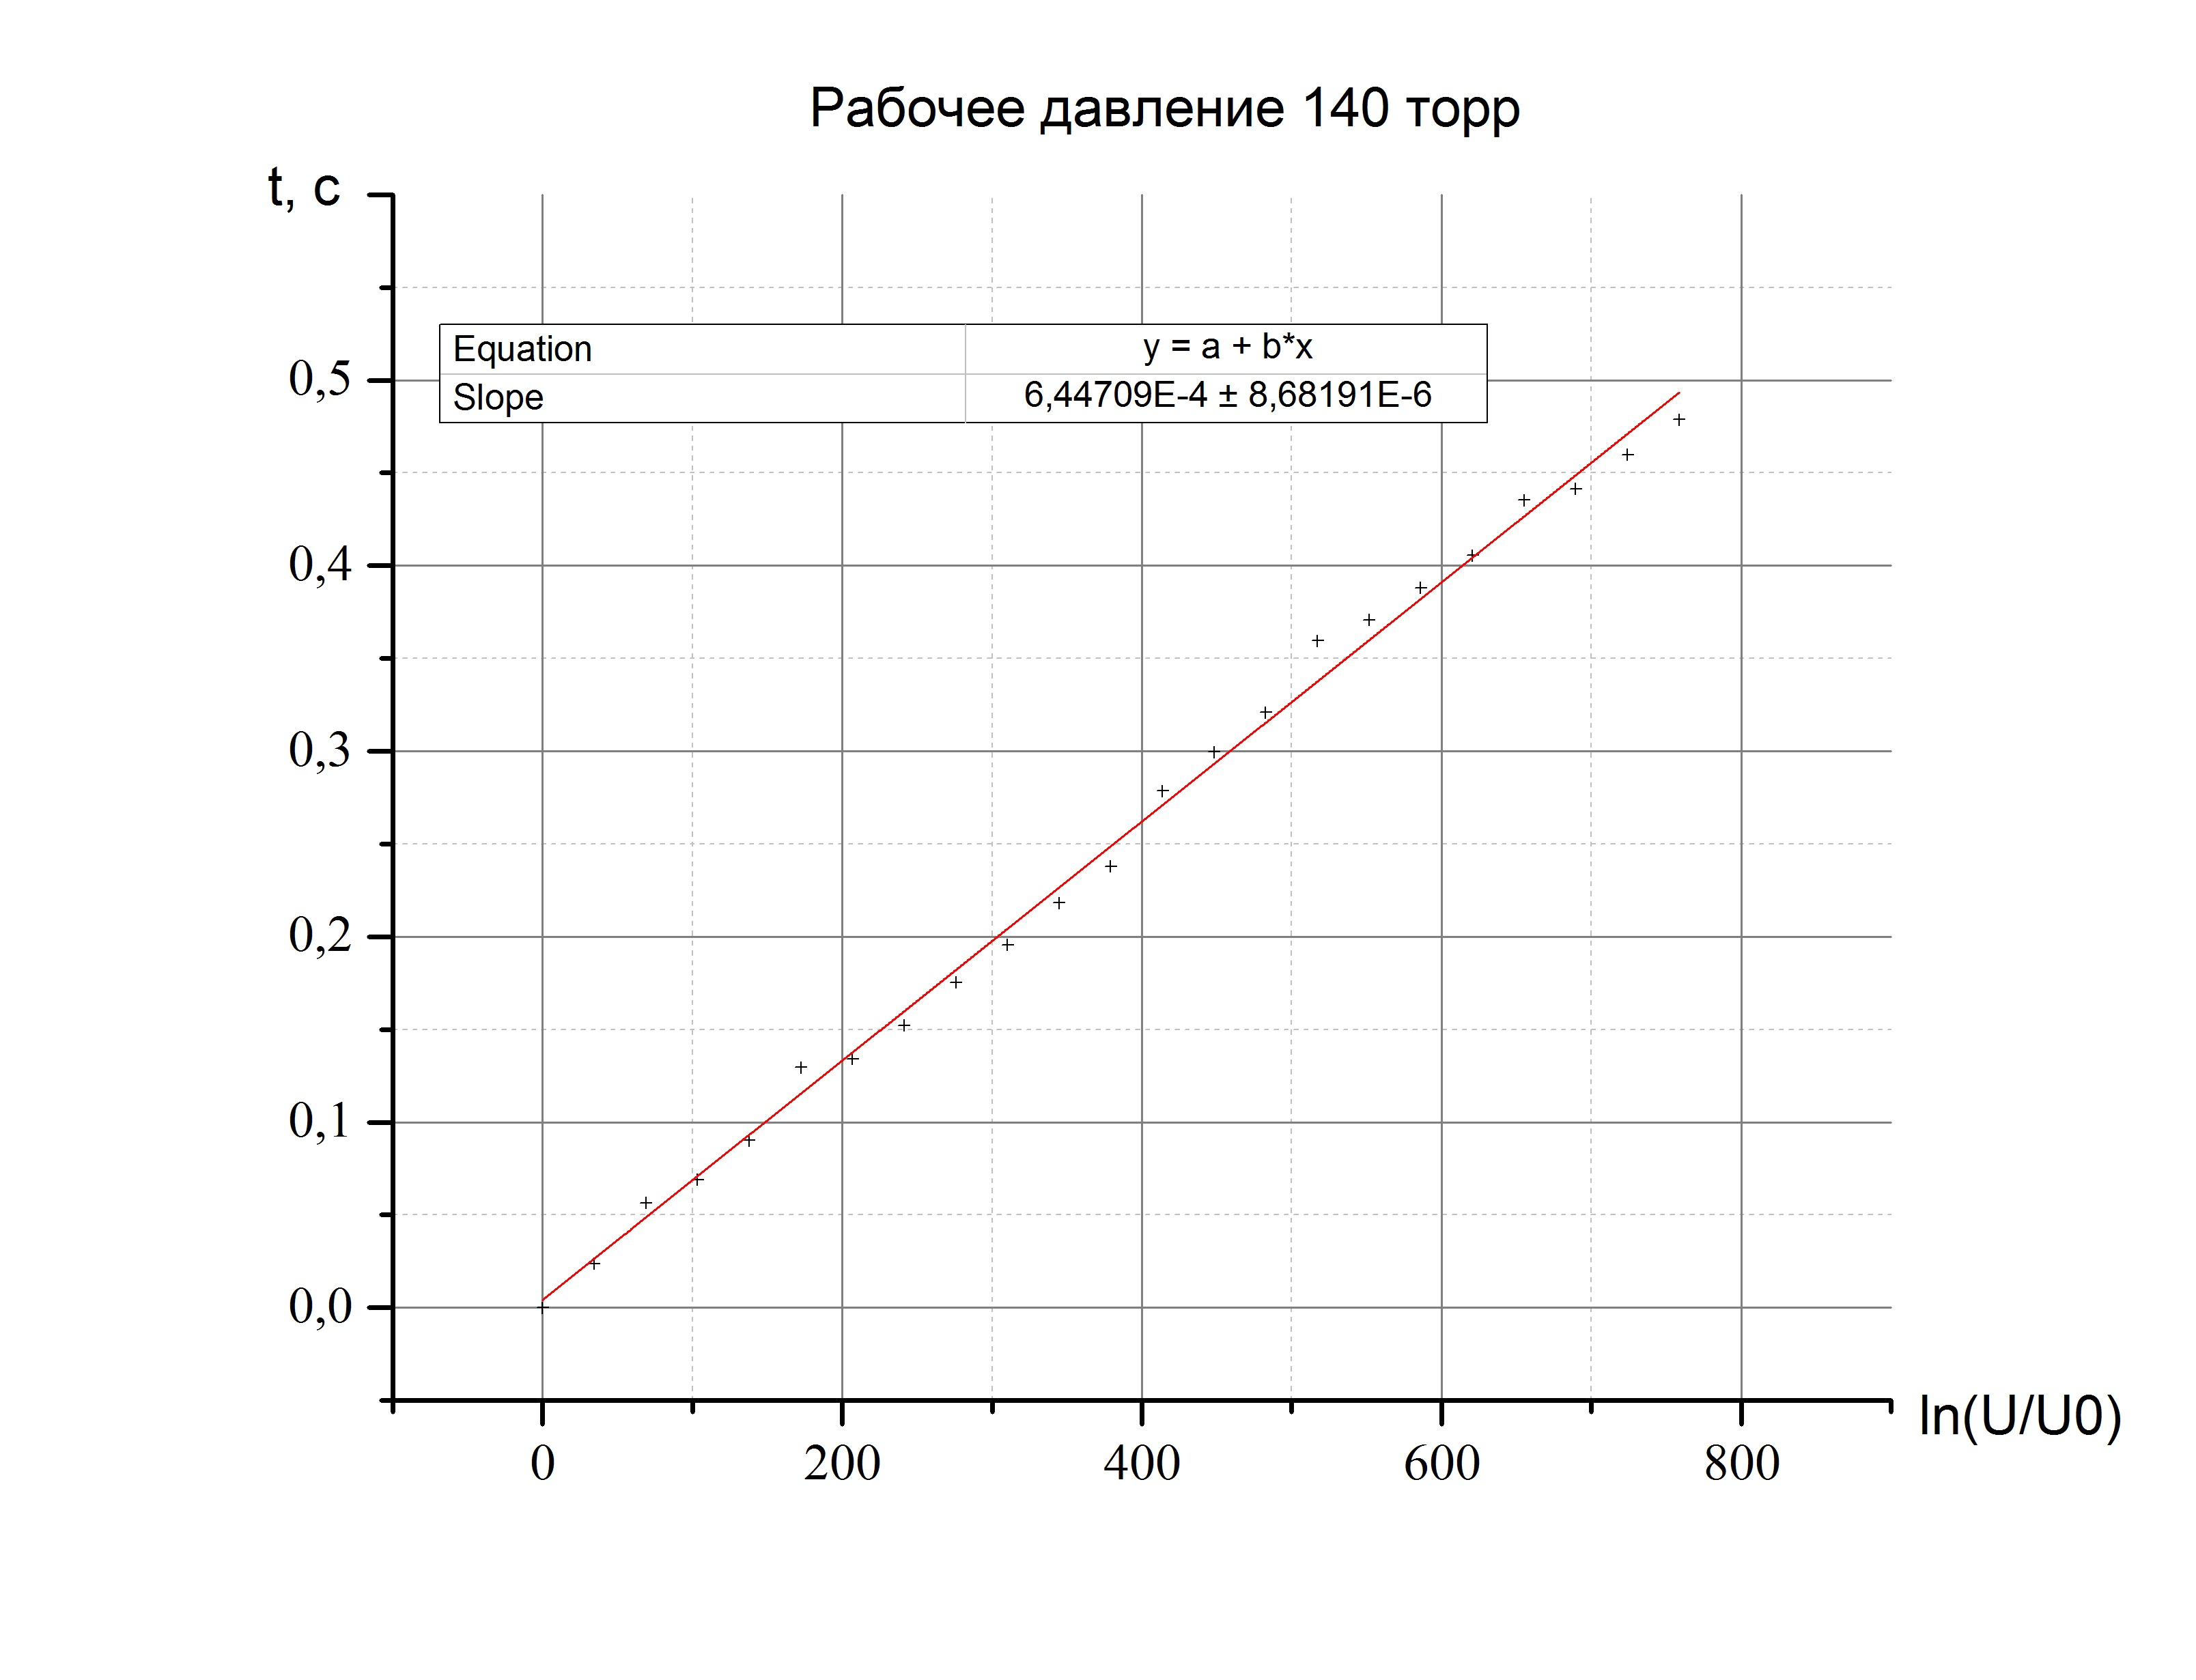
\includegraphics[scale=0.55]{Graph8.jpg}\\
\newpage
Получаем, что\\
\ \\
\begin{tabular}{|c|c|}
\hline 
P рабочее, торр & D, см$^2$/c \\ 
\hline 
40 & $7,2\pm 0,6$ \\ 
\hline 
75 & $4,1\pm 0,4$ \\ 
\hline 
140 & $2,1\pm 0,2$ \\ 
\hline 
180 & $1,72\pm 0,2$ \\ 
\hline 
\end{tabular} \\
\ \\
\begin{center}
Теперь построим график D(1/P)
\end{center}
\ \\
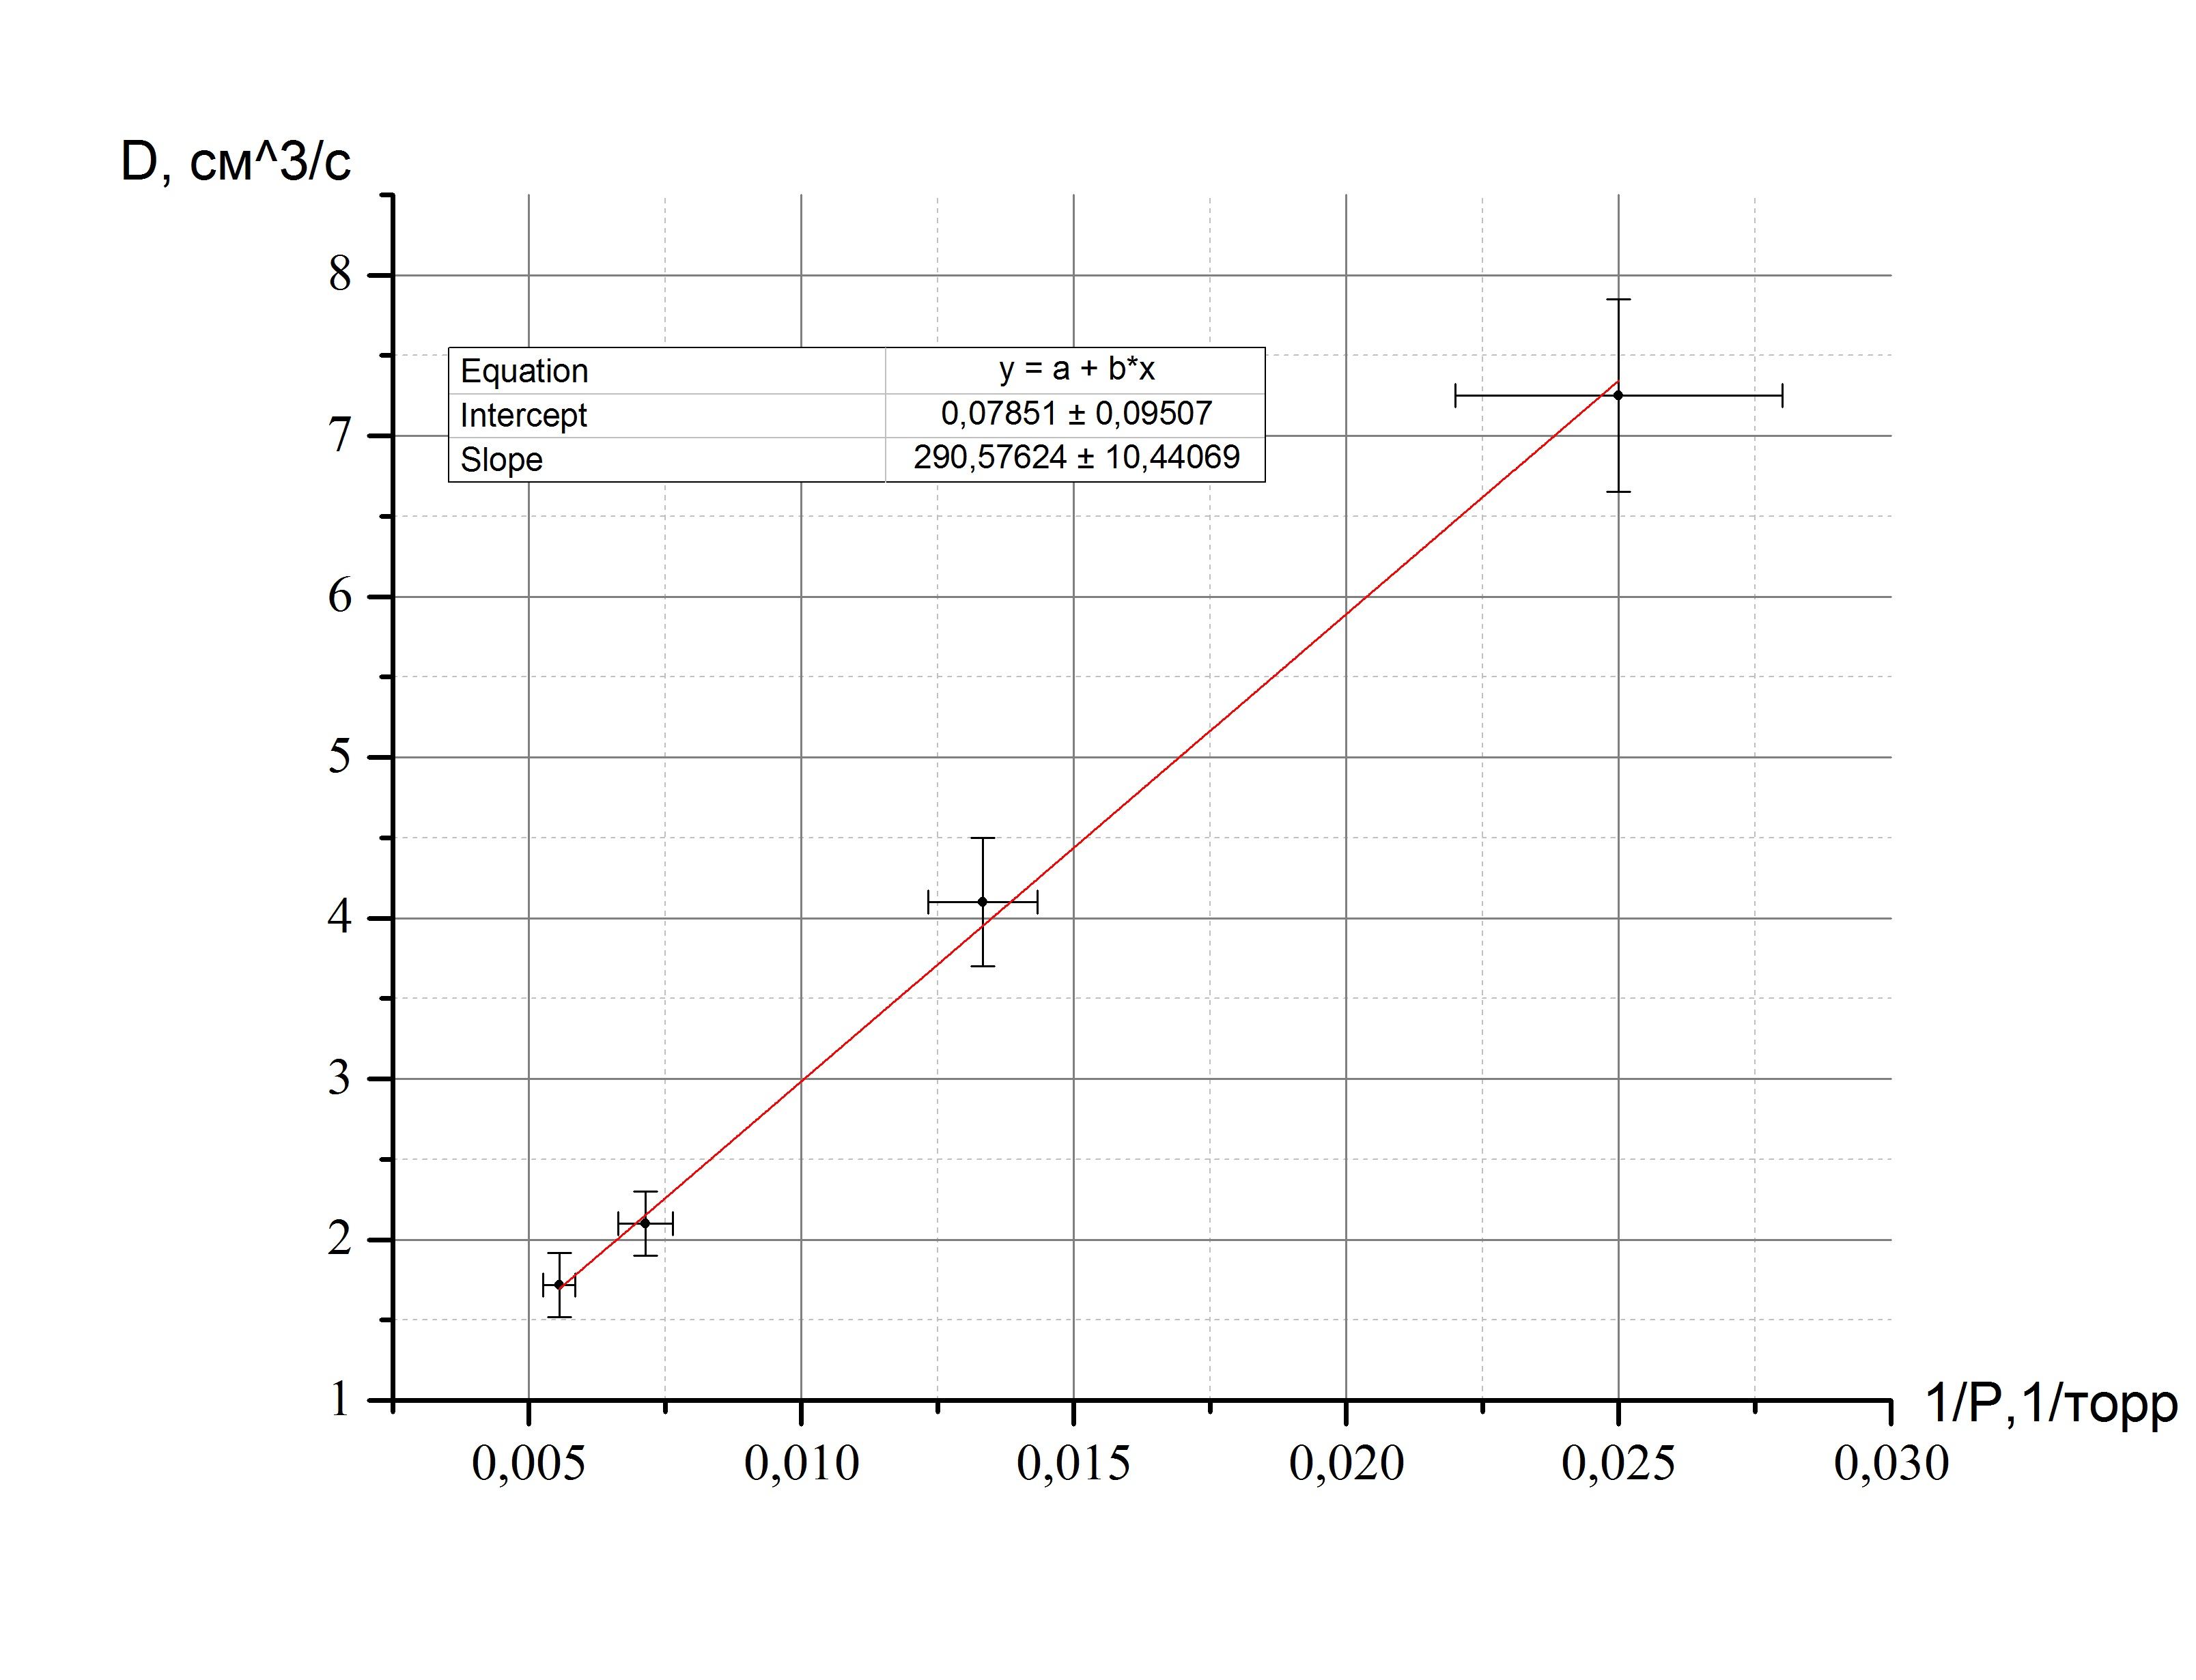
\includegraphics[scale=0.6]{Graph9.jpg}\\
Тогда, проэкстраполировав к P=757 торр, получим, что $D=(0,46\pm 0,07)$ см$^2$/c
\ \\
$D=\frac{1}{3}\lambda <v>, <v>=\sqrt{\frac{8RT}{\pi M}}$ \\
Тогда $\lambda\approx 10^{-7}$ м; $\sigma\approx4*10^{-19}$ м$^2$
\noindent 
\ \\
\ \\
\ \\
\ \\
\indent \subsubsection*{Литература}
Лабораторный практикум по общей физике. Термодинамика/А.Д. Гладун - М, 2004 г\\
\end{document}